% Created 2024-06-23 Sun 22:37
% Intended LaTeX compiler: pdflatex
\documentclass[11pt]{article}
\usepackage[utf8]{inputenc}
\usepackage[T1]{fontenc}
\usepackage{graphicx}
\usepackage{longtable}
\usepackage{wrapfig}
\usepackage{rotating}
\usepackage[normalem]{ulem}
\usepackage{amsmath}
\usepackage{amssymb}
\usepackage{capt-of}
\usepackage{hyperref}
\author{Eduardo Lemos}
\date{23/06/2024}
\title{Projeto 2 | Rusting Images}
\hypersetup{
 pdfauthor={Eduardo Lemos},
 pdftitle={Projeto 2 | Rusting Images},
 pdfkeywords={},
 pdfsubject={},
 pdfcreator={Emacs 29.3 (Org mode 9.6.15)}, 
 pdflang={English}}
\begin{document}

\maketitle
\tableofcontents

O projeto foi desenvolvido na linguagem Rust, com o package manager \texttt{cargo}.
Todos os exemplos descritos utilizaram a imagem \texttt{./assets/kodim03.png} como base.

\begin{center}
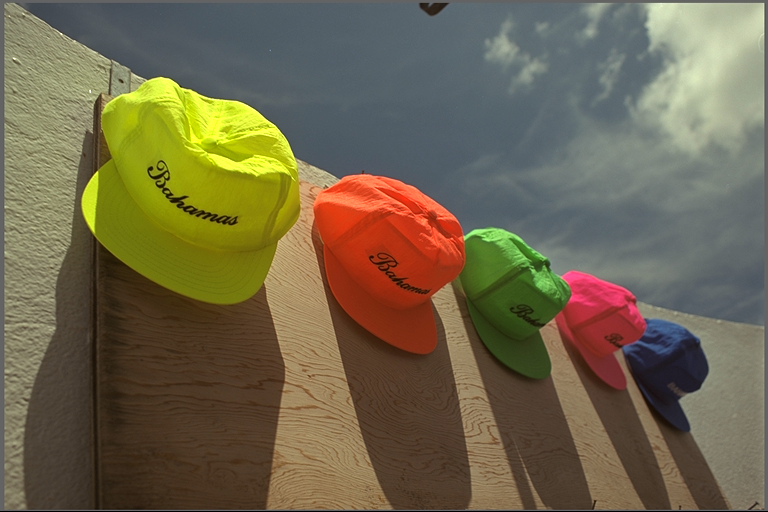
\includegraphics[height=0.4\textwidth]{../assets/kodim03.png}
\end{center}

\section{C1}
\label{sec:org92e68be}

O codec C1 apenas binariza imagem detectando qual valor, em escala de cinza, o pixel mais se aproxima. Caso
esteja mais próximo de 255 do que de 0, o pixel se torna branco e vice-versa.

Na linha de comando:

\begin{verbatim}
[user@nixos:/rusting-images]$ cargo run -- c1 ./assets/kodim03.png
Loading image...
Image loaded!
Applying C1 codec...
Calculated Average PSNR: 8.27 dB
Saving image...
\end{verbatim}

\begin{center}
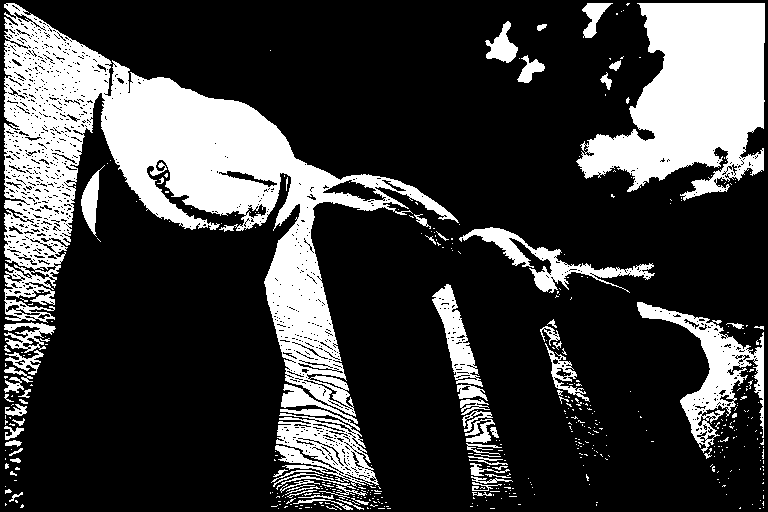
\includegraphics[height=0.4\textwidth]{../assets/kodim03_c1.png}
\end{center}

Em teoria, a taxa \emph{bpp} do codec C1 é 1 bit por pixel. Porém, como cada pixel da imagem gerada
está em RGB, a taxa sobe para 24 bits por pixel.

\section{C2}
\label{sec:org01e4d79}

O codec C2 aplica a estratégia de Dithering na em uma imagem em escala de cinza. A partir de uma
máscara para o Dithering, a imagem é percorrida e é calculado a diferença entre o pixel original
da imagem (em escala de cinza) e o novo pixel (que no nosso caso é obtido a partir da estratégia
de limiar descrita em C1). Essa diferença, ou erro, é propagada para os pixels vizinhos utilizando-se
da máscara provida. Em caso padrão, essa máscara será a de \href{https://en.wikipedia.org/wiki/Floyd\%E2\%80\%93Steinberg\_dithering}{Floyd-Steinberg}. O codec C2 binariza
a imagem final obtida utilizando a mesma estratégia descrita em C1, obtendo-se uma imagem com
apenas pixels pretos ou brancos.

Na linha de comando:

\begin{verbatim}
[user@nixos:/rusting-images]$ cargo run -- c2 ./assets/kodim03.png
Loading image...
Image loaded!
Applying C2 codec...
Calculated Average PSNR: 6.44 dB
Saving image...
\end{verbatim}

\begin{center}
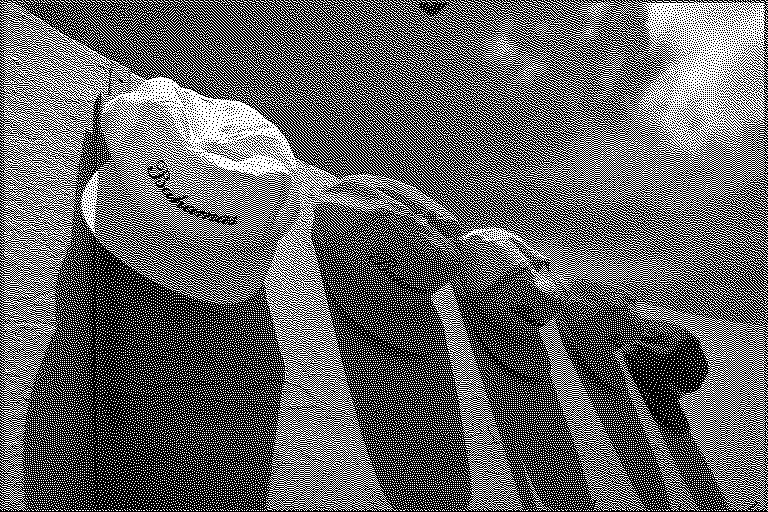
\includegraphics[height=0.4\textwidth]{../assets/kodim03_c2.png}
\end{center}

Nota-se que o valor PSNR calculado é menor que o encontrado no codec C1. Isso é esperado pois
o processo de Dithering \textbf{propositalmente} inclúi extra ruído para obter uma imagem com melhor visual
subjetivamente.

Em teoria, a taxa \emph{bpp} do codec C2, assim como C1, é 1 bit por pixel. Porém, como cada pixel da imagem gerada
está em RGB, a taxa sobe para 24 bits por pixel.

\section{CIMap}
\label{sec:org1201df9}

O codec CIMap utiliza quantização vetorial para diminuir a palheta de cores da imagem utilizando-se
o algoritmo LBG. O processo começa com a escolha de um codebook inicial a partir dos pixels
iniciais da imagem. Em seguida, inicia-se o processo de \emph{clustering}, isto é, o cálculo iterativo
para o encontro dos melhores \emph{centroides} para uma dada imagem.

Esse processo se baseia em alcançar convergência entre o conjunto de centroides atuais e melhores
candidatos. Cada pixel será mais próximo de um dos centroides disponíveis e um novo centroide
é encontrado após todos os pixels serem mapeados com qual centroide atual eles estão mais próximos.
Quando esse processo convergir, os centroides finais serão a palheta de cores que utilizaremos para
pintar a imagem final.

Na linha de comando (para 16 cores):

\begin{verbatim}
[user@nixos:/rusting-images]$ cargo run -- ci-map ./assets/kodim03.png 16
Loading image...
Image loaded!
Applying CIMap codec...
Calculated Average PSNR: 22.66 dB
Saving image...
\end{verbatim}

\subsection{Comparação com JPEG}
\label{sec:org832d1ad}

Devemos comparar os valores PSNR com os valores de bits por pixel ou \emph{bpp} do nosso codificador
com um codificador JPEG de tamanho teórico aproximado. Em teoria, o valor bpp que cada quantizador vetorial com um
codebook de \(C\) centroides com tamanho \(N*M\) deve gerar segue a seguinte fórmula:

$$ codebookSize = 24 bits * C $$
$$ bpp = \frac{NM \log_2 C + codebookSize}{NM} $$
$$ bpp = \frac{NM \log_2 C + 24C}{NM} \approx \log_2 C $$

Destaca-se que para o codificador JPEG a taxa bpp sempre será de 24 bits por pixel, porém será codificado a imagem em JPEG assumindo
o tamanho teórico estabalecido pela fórmula acima (valores aproximados usando a ferramenta GIMP). A seguinte fórmula determina qual
deve ser o tamanho aproximado para o JPEG em bytes:

$$ JPEG = NM \log_2 C $$

O cálculo da PSNR para quaisquer imagens pode ser obtido pela linha de comando:

\begin{verbatim}
[user@nixos:/rusting-images]$ cargo run -- psnr kodim03.png kodim03_32.jpg
Loading image...
Image loaded!
Loading image...
Image loaded!
Calculated Average PSNR: 46.51 dB
\end{verbatim}

Finalmente, o gráfico a seguir compara os dois codificadores:

\begin{center}
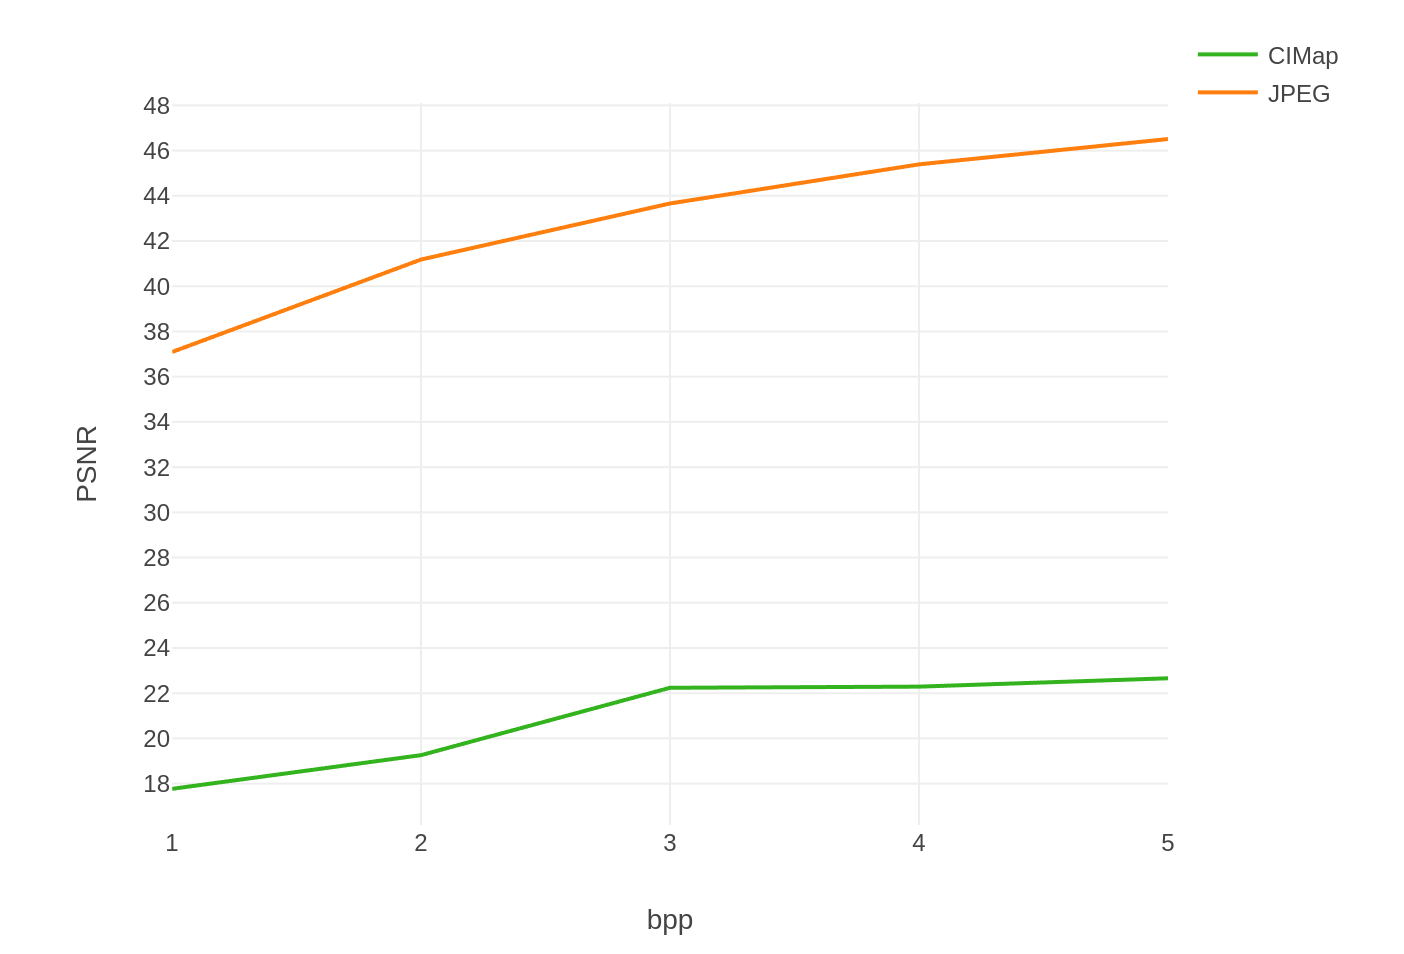
\includegraphics[height=0.8\textwidth]{./graph.png}
\end{center}

A seguir os pares de imagem com o JPEG e CIMap para (aproximadamente) o mesmo valor bpp:

\begin{center}
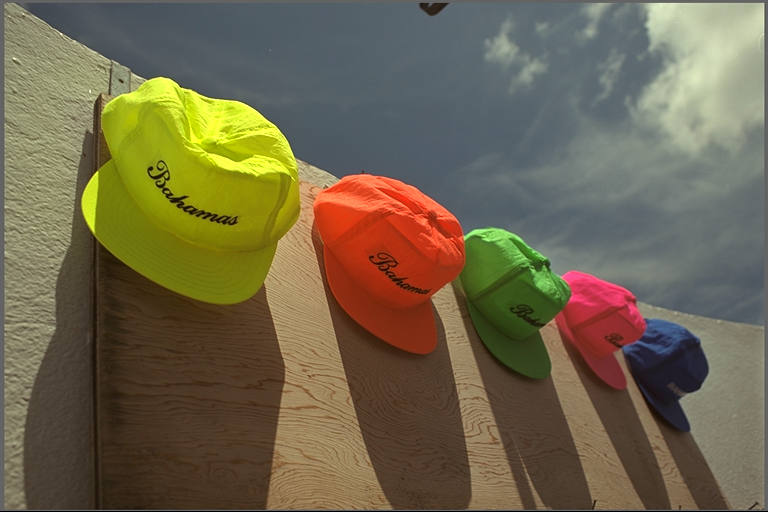
\includegraphics[height=0.3\textwidth]{../assets/kodim03_2.jpg}
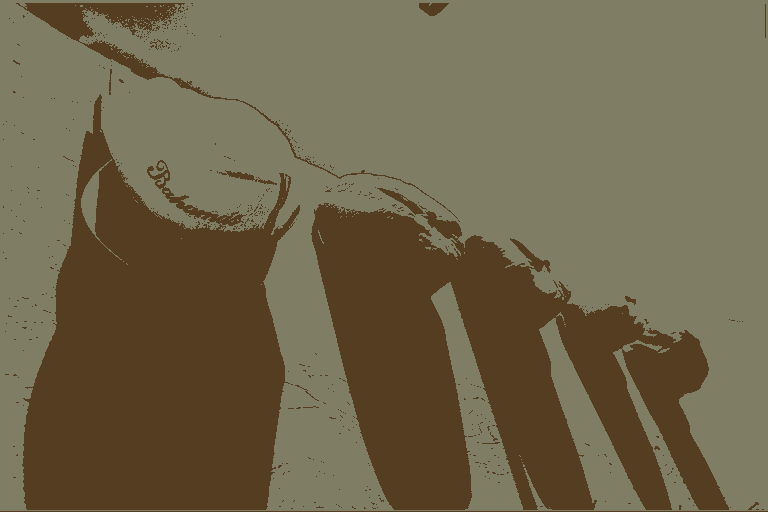
\includegraphics[height=0.3\textwidth]{../assets/kodim03_cimap_2.png}
\end{center}

\begin{center}
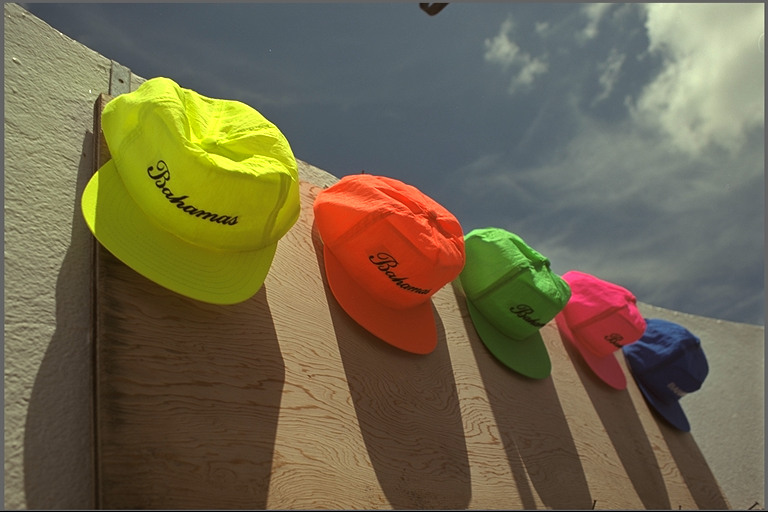
\includegraphics[height=0.3\textwidth]{../assets/kodim03_4.jpg}
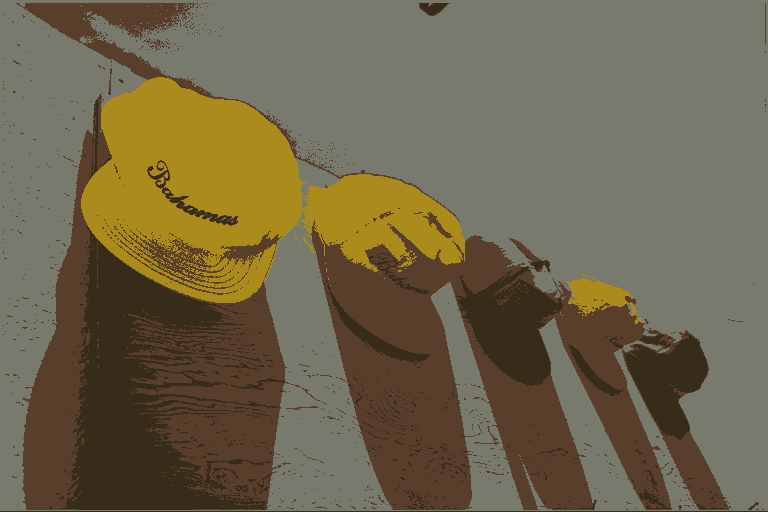
\includegraphics[height=0.3\textwidth]{../assets/kodim03_cimap_4.png}
\end{center}

\begin{center}
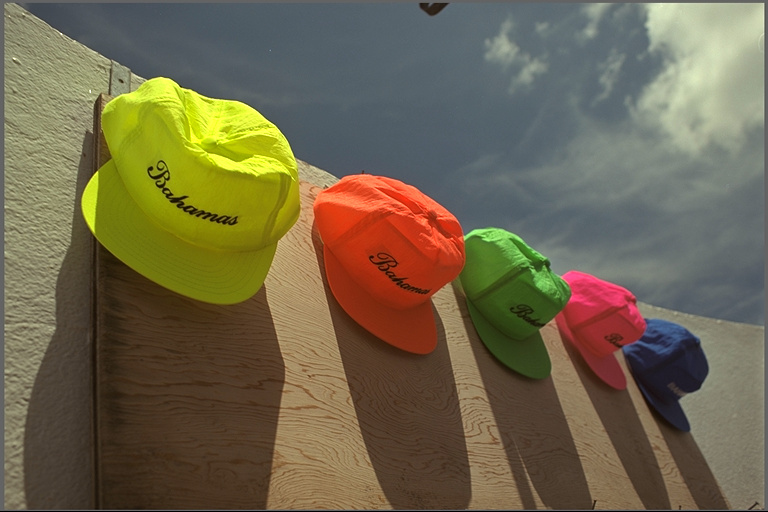
\includegraphics[height=0.3\textwidth]{../assets/kodim03_8.jpg}
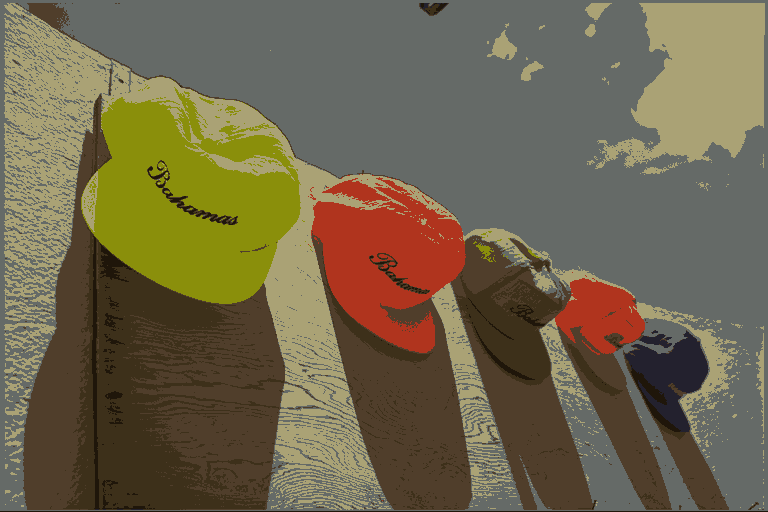
\includegraphics[height=0.3\textwidth]{../assets/kodim03_cimap_8.png}
\end{center}

\begin{center}
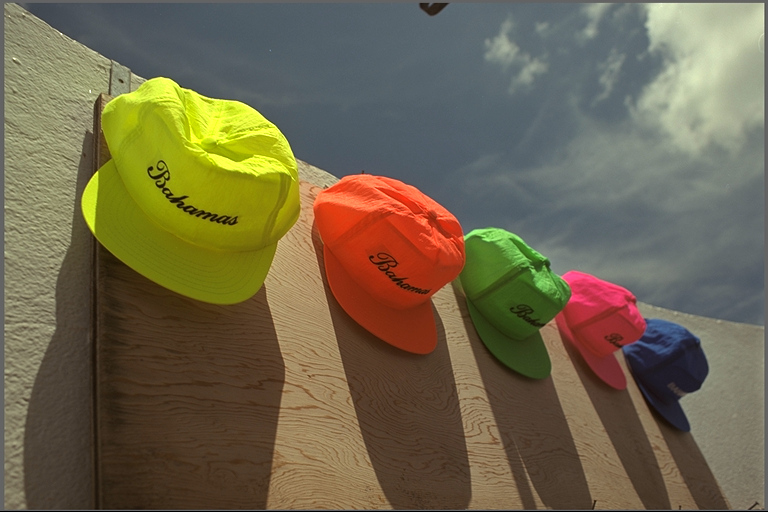
\includegraphics[height=0.3\textwidth]{../assets/kodim03_16.jpg}
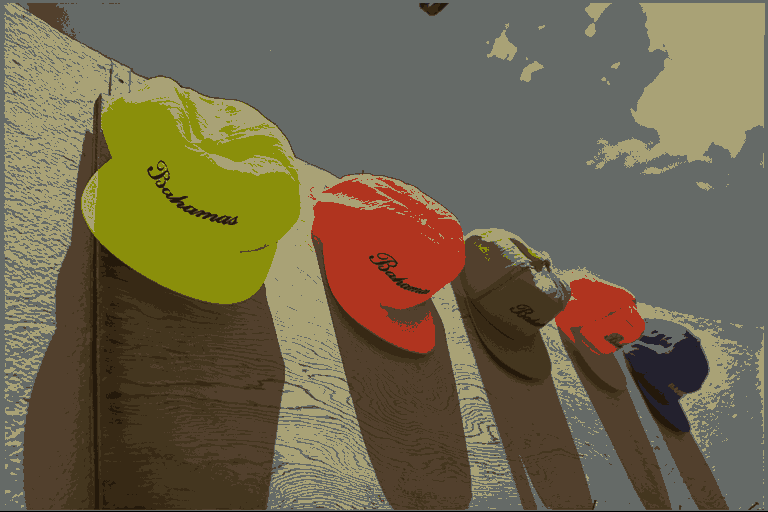
\includegraphics[height=0.3\textwidth]{../assets/kodim03_cimap_16.png}
\end{center}

\begin{center}
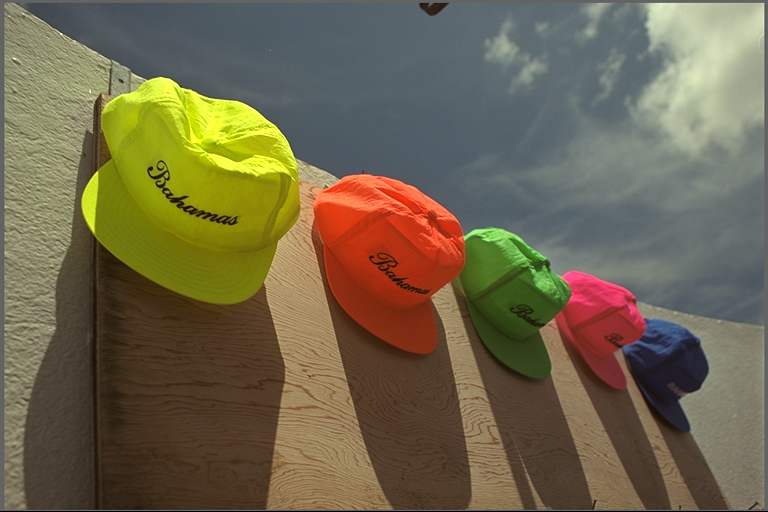
\includegraphics[height=0.3\textwidth]{../assets/kodim03_32.jpg}
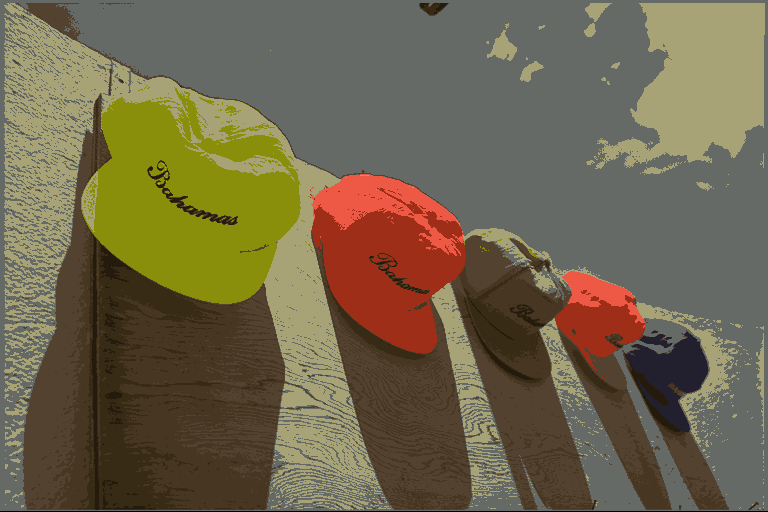
\includegraphics[height=0.3\textwidth]{../assets/kodim03_cimap_32.png}
\end{center}

\section{CIMap2}
\label{sec:orga467619}

O codec CIMap2 é uma união dos codecs C2 e CIMap, isto é, devemos aplicar a estratégia de dithering
em uma imagem colorida que tenha sido quantizada pela quantização vetorial. Isso foi feito da seguinte
forma: quantiza-se a imagem e para cada canal da imagem, e.g., R, G, B, aplicou-se o dithering de Floyd-Steinberg.
A imagem final será composta dos 3 canais unidos após suas transformações individuais.

Na linha de comando (para 16 cores):

\begin{verbatim}
[user@nixos:/rusting-images]$ cargo run -- ci-map ./assets/kodim03.png 16
Loading image...
Image loaded!
Applying CIMap2 codec...
Calculated Average PSNR: 6.75 dB
Saving image...
\end{verbatim}

\begin{center}
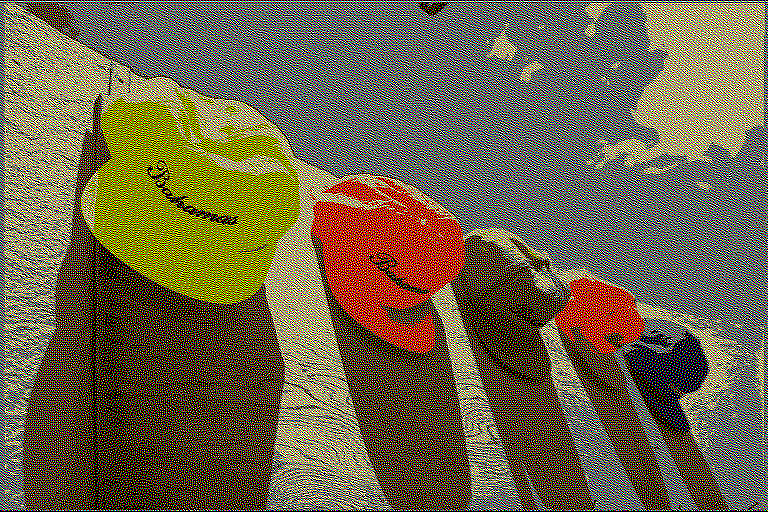
\includegraphics[height=0.4\textwidth]{../assets/kodim03_cimap2.png}
\end{center}

Nota-se que, assim como no codec C2 em relação a C1,  o valor PSNR calculado é menor que o encontrado no codec CIMap.
Isso é esperado pois o processo de Dithering \textbf{propositalmente} inclúi extra ruído para obter uma imagem com melhor visual
subjetivamente.

\section{Melhorias}
\label{sec:org98c4150}

A principal melhoria que poderia ser implementada seria o uso de concorrência em codecs como
CIMap para acelerar sua execução.
\end{document}
